\section{Aufgabenteil 3}
Im dritten Aufgabenteil der \"Ubung geht es darum das berechnete Schwerefeld einer approximierten Kugel mit der analytischen L\"osug zu vergleichen. Hierbei beziehen wir uns auf das Paper {\it gravity and magnetic fields of polygonal prisms and application to magnetic terrain corrections} von Plouff (1976), in dem die Schwerewirkung eines n-eckigen Polygons berechnet wird. \\
Die Kugel (mit $R=2m$ bei [0 0 4m]) in unserem Modell soll durch k Schichten n-eckiger Polygone angen\"ahert werden und den Dichteunterschied $\delta \rho =200 \frac{kg}{m^{3}}$ zu der Umgebung aufweisen. In Abbildung \ref{fig:kugel} ist eine durch 100 Schichten von 100-eckigen Polygonen approximierte Kugel zu erkennen. Optisch ist bei einer Abtastung durch viele Polygonecken und Schichten kein Unterschied zu einer Kugel zu erkennen. Es gilt nun festzustellen, wie stark das Schwerefeld von der Anzahl der Schichten und Polygonecken abh\"angt.\\

\begin{figure}[h]
\begin{center}
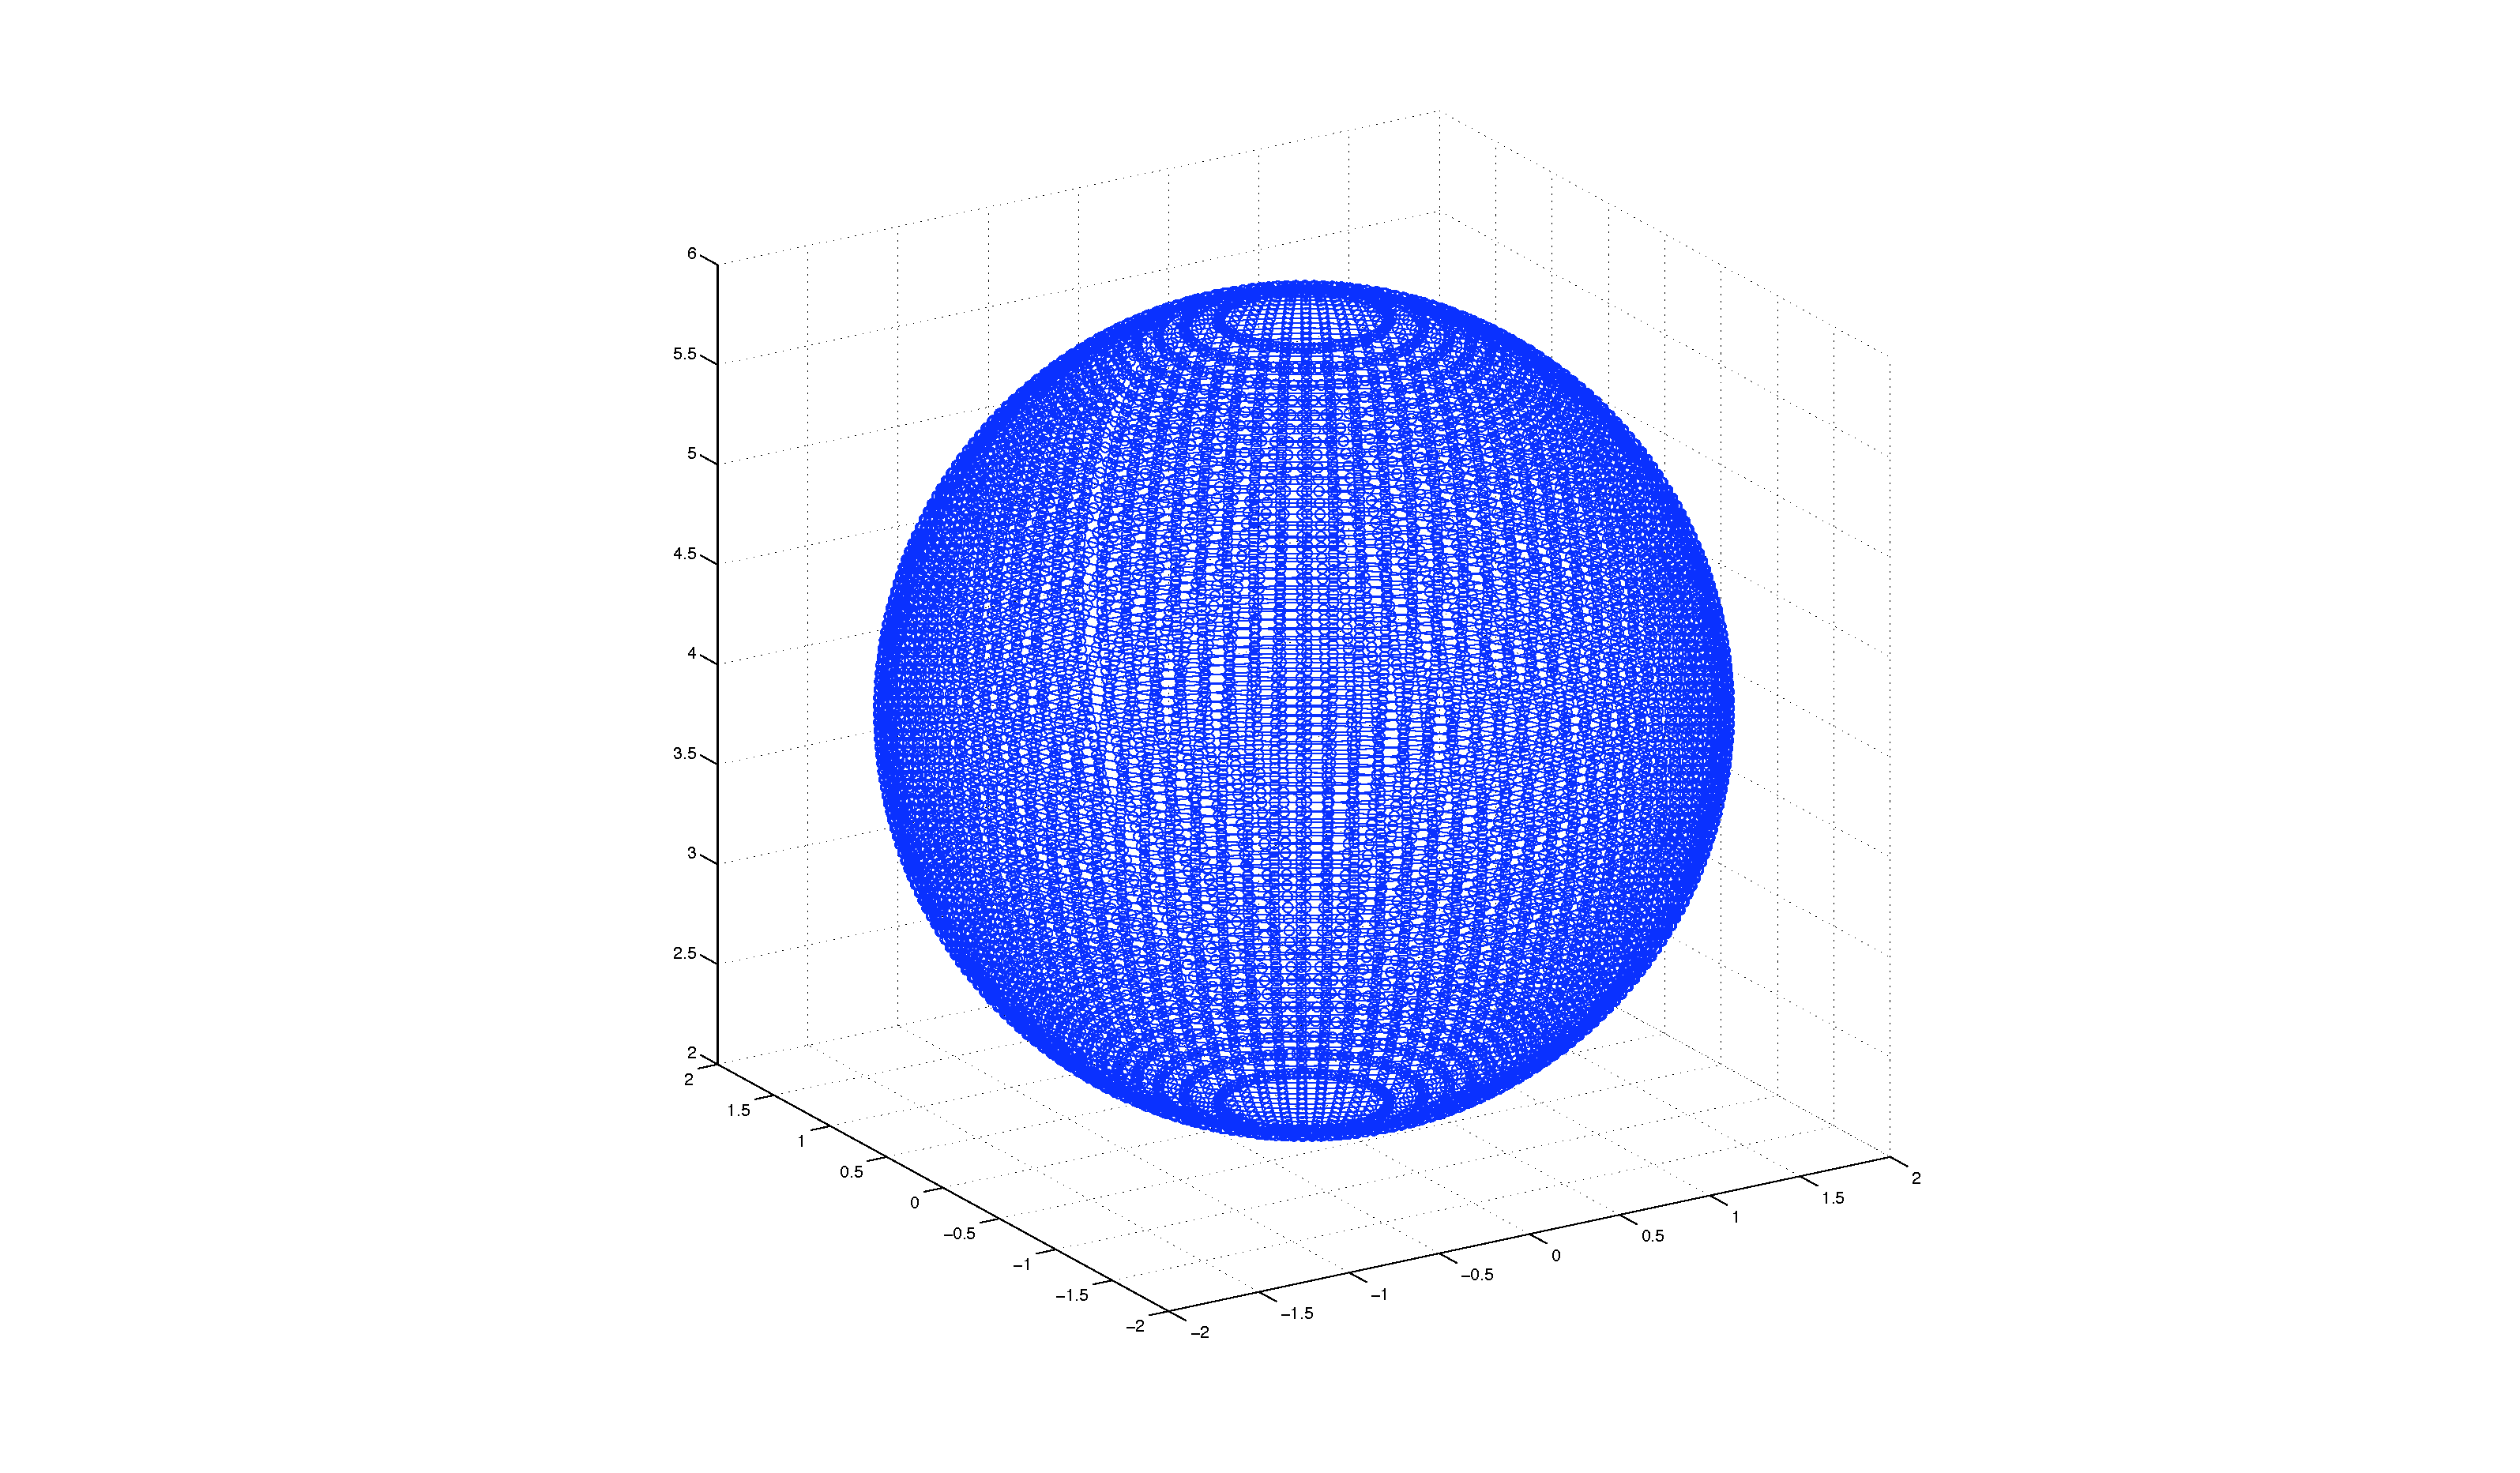
\includegraphics[scale=0.5]{Plots/Kugel.pdf}
\caption{Approximierte Kugel aus 100 Schichten und 100-eckigen Polygonen}
\label{fig:kugel}
\end{center}
\end{figure}

\noindent
Um die Schwere zu berechnen wird die Schwerebeschleunigung aller Kanten und aller Polygone aufsummiert. Daf\"ur wird die von Plouff (1976) eingef\"uhrte Formel verwendet (3) verwendet.\\



\begin{equation}
g = \gamma \rho s_{m} \sum_{i=1}^{n} \bigg\{ s_{p}  A (z_{1}-z_{2})
%\end{equation}
%\begin{equation}
+ z_{2} \Big( tan^{-1}(\frac{z_{2} d_{1}}{PR_{12}})- tan^{-1}(\frac{z_{2} d_{2}}{P R_{22}})\Big) %\nonumber
\end{equation}
\begin{equation}
- z_{1}\Big( tan^{-1}(\frac{z_{1} d_{1}}{P R_{11}}) - tan^{-1}(\frac{z_{1} d_{2}}{P R_{21}} \Big) %\nonumber
%\end{equation}
%\begin{equation}
- P \cdot ln(\frac{R_{22}+d_{2}}{R_{12}+d_{1}} \frac{R_{11}+d_{1}}{R_{21}+d_{2}}) \bigg\}  \nonumber
\end{equation}



\noindent
Die analytische L\"osung ergibt sich aus der Schwerebeschleunigung einer Punktmasse M
\begin{equation}
g=-\frac{\gamma \cdot M}{r^{2}}
\end{equation}
mit
\begin{equation}
M=-\frac{4}{3} \pi R^{3} d\rho
\end{equation}


\noindent
Abbildung \ref{fig:analkugel} zeigt die analytische L\"osung f\"ur das Schwerefeld der Kugel. Die Form und Gr\"o\ss enordnung stimmt weitestgehend mit der approximierten L\"osung in Abbildung \ref{fig:approx} \"uberein. Bei genauerer Betrachtung f\"allt jedoch auf, dass die Schwerebeschleunigung bei zunehmendem Abstand zum Mittelpunkt bei der analytischen L\"osung wesentlich schneller abflacht. Dieser Effekt r\"uhrt vermutlich daher, dass bei der analytischen L\"osung von einer Punktmasse in der Mitte der Kugel ausgegangen wird. Der Abstand zur Kugel geht demnach als Abstand zum Mittelpunkt der Kugel ein. 

\newpage

% Aus irgendeinem Grund nimmt er bei mir die Referenzen von den Abbildungen nicht richtig... wei� nicht was da los ist.

\begin{figure}[h]
\begin{center}
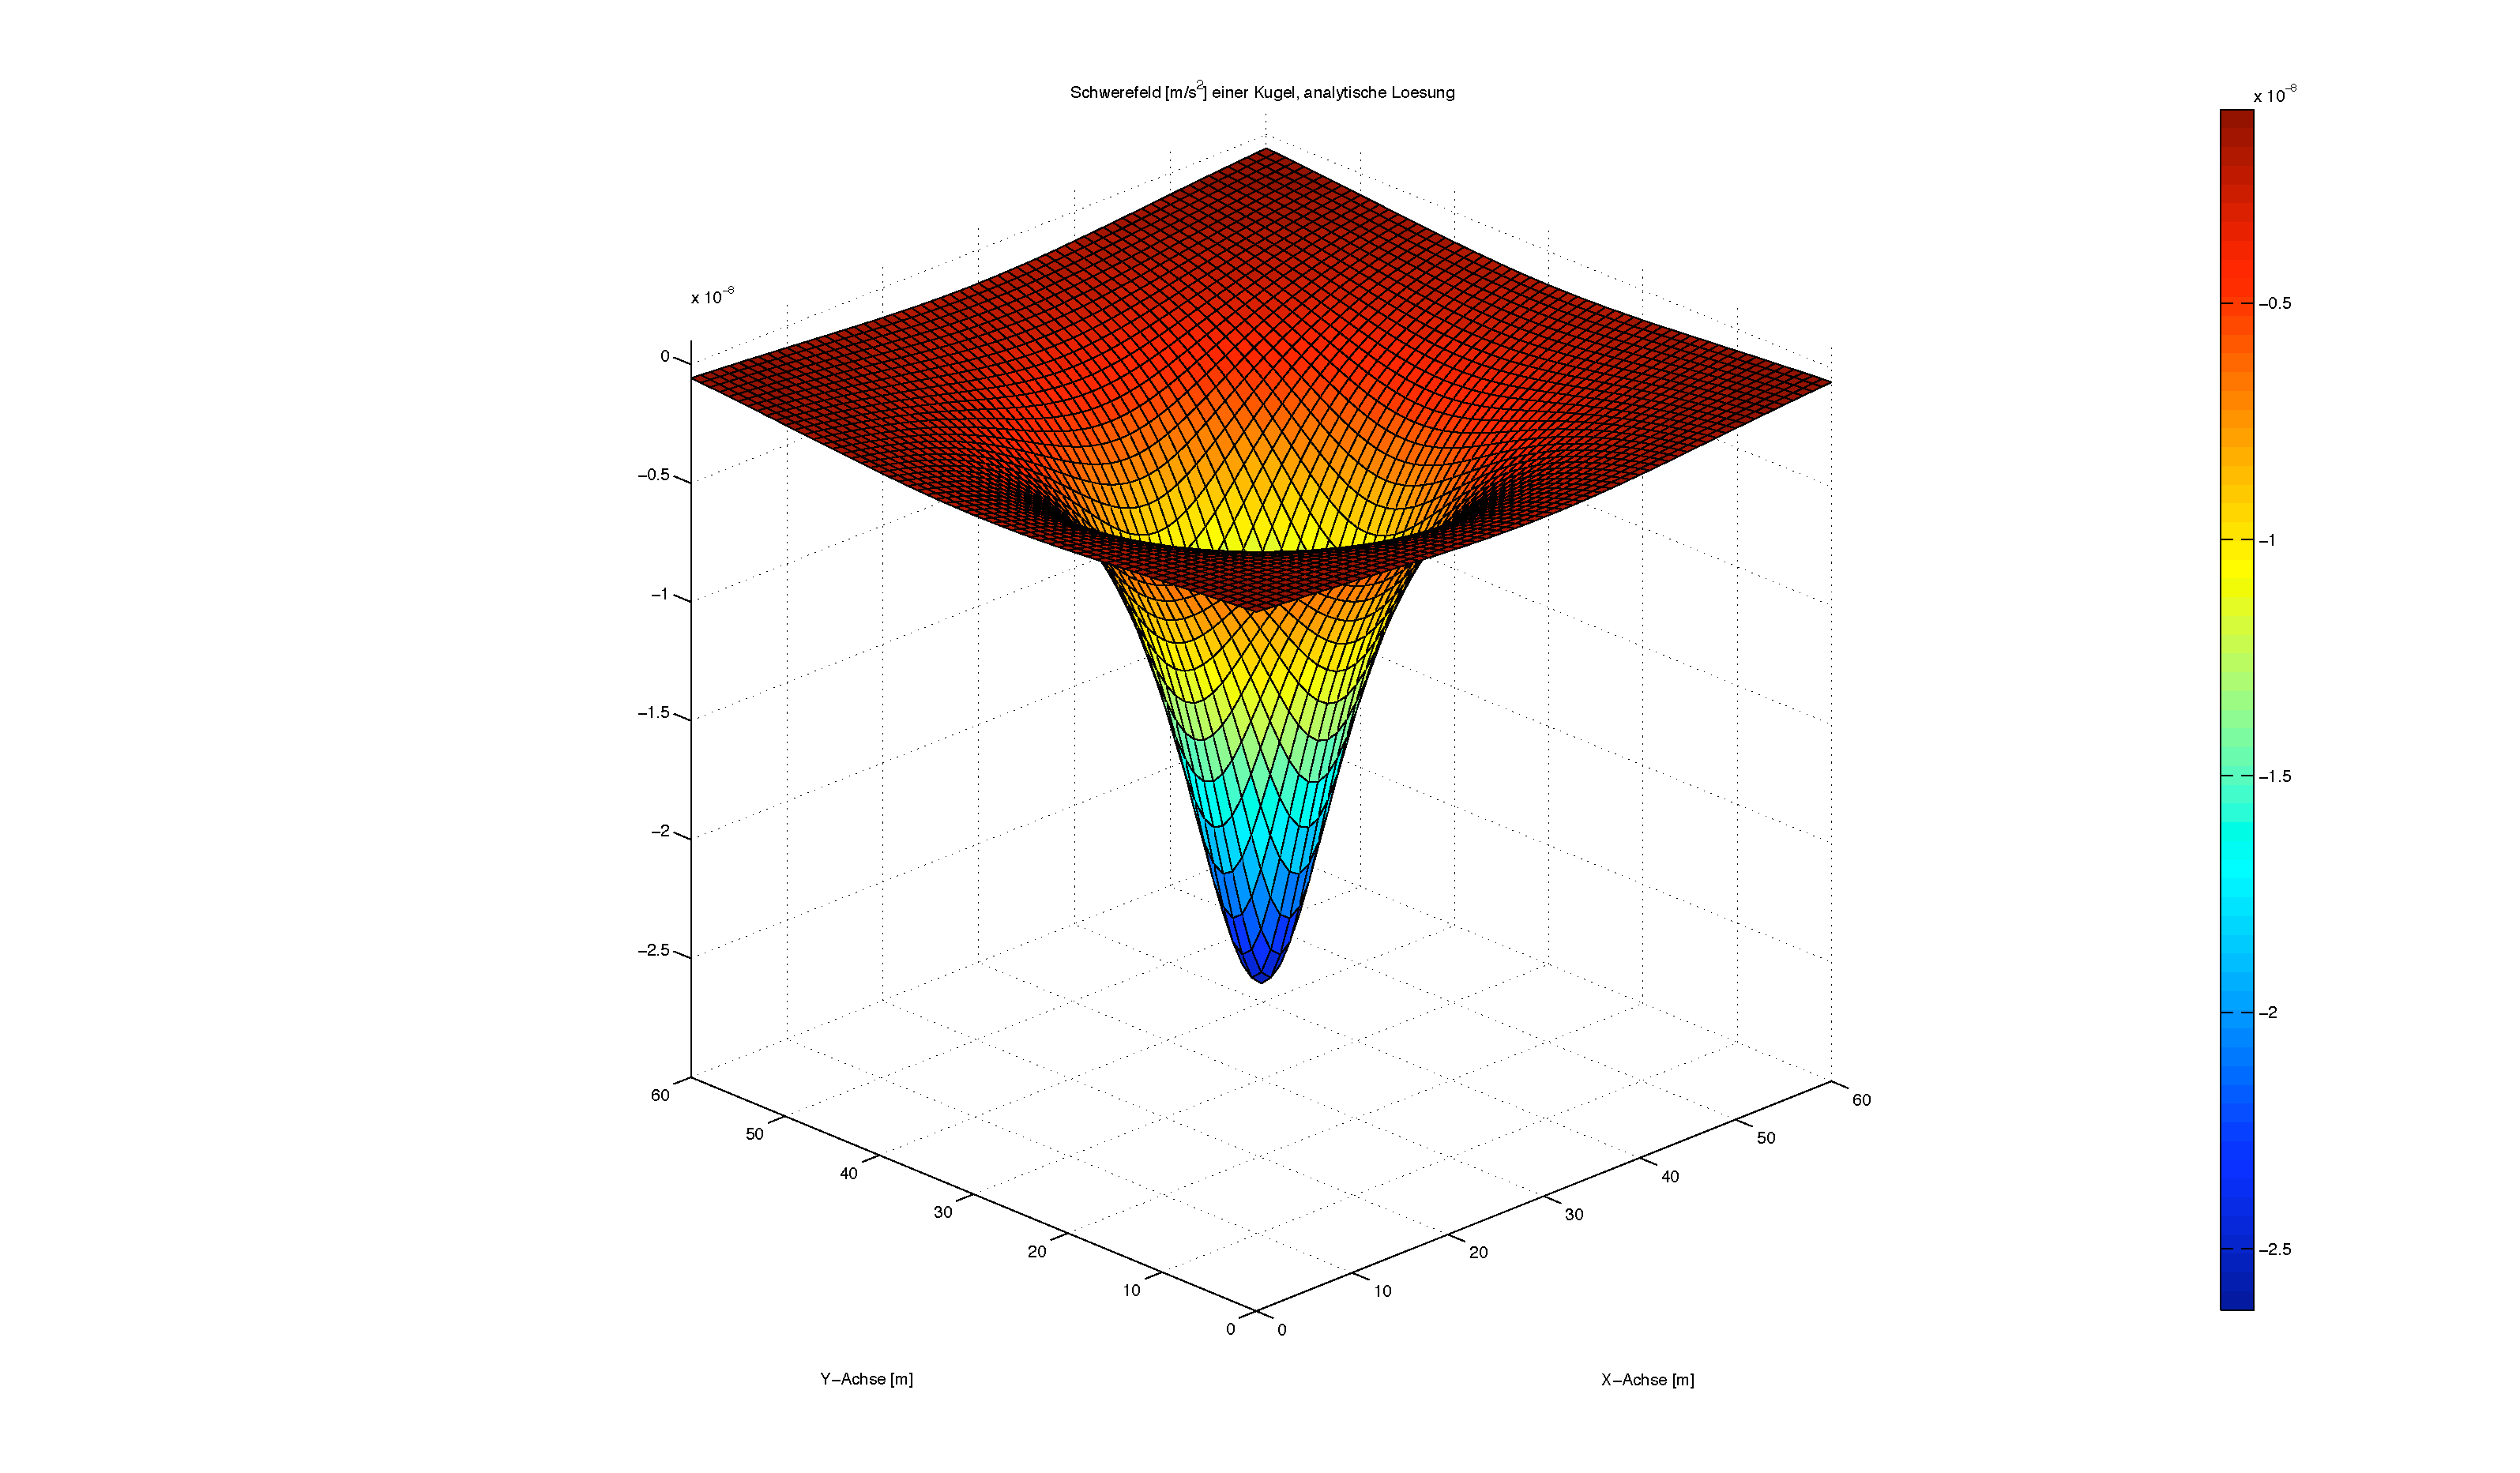
\includegraphics[scale=0.3]{Plots/AnalytischeLsgKugel.pdf}
\caption{analytische L\"osung f\"ur das Schwerefeld einer Kugel}
\label{fig:analkugel} % was fuern witz... HarHarHar!!
\end{center}
\end{figure}

\begin{figure}[h]
\begin{center}
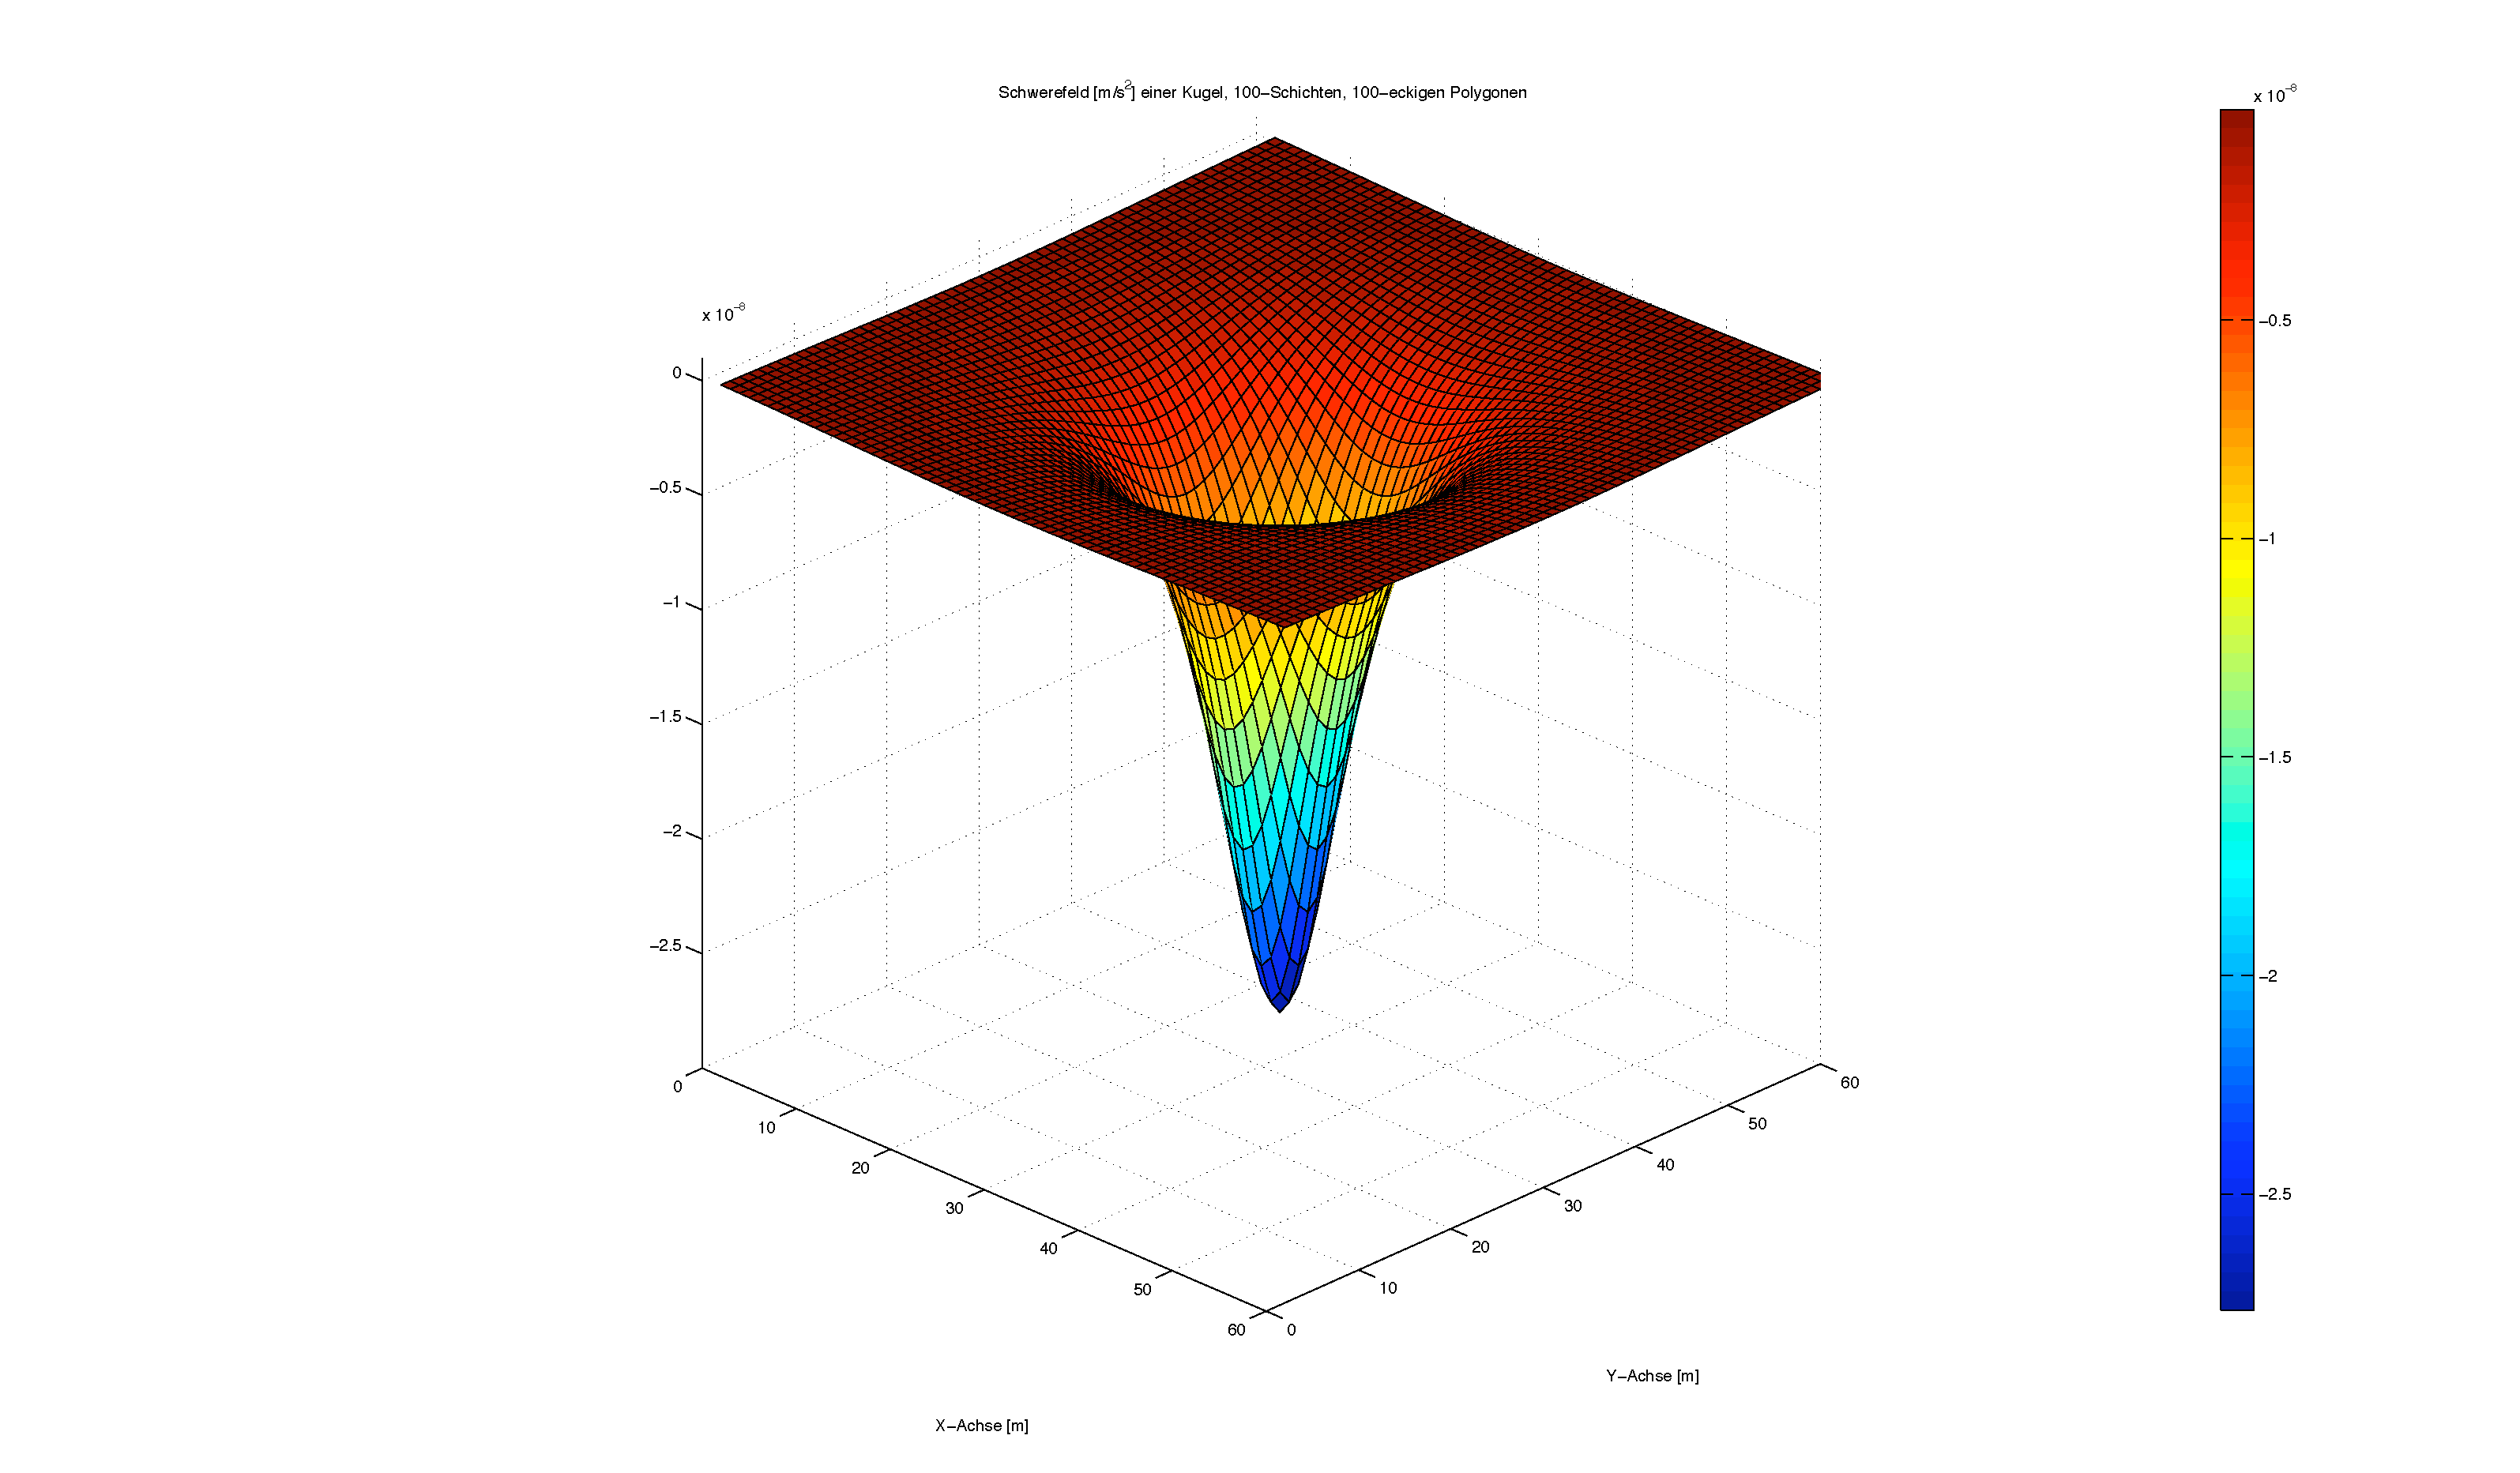
\includegraphics[scale=0.3]{Plots/ApproxKugelSchwere.pdf}
\caption{Schwerefeld einer durch 100 Schichten 100-eckeniger Polygonen approximierten Kugel}
\label{fig:approx}
\end{center}
\end{figure}

\newpage
bla bla

\begin{figure}[h]
\begin{center}
%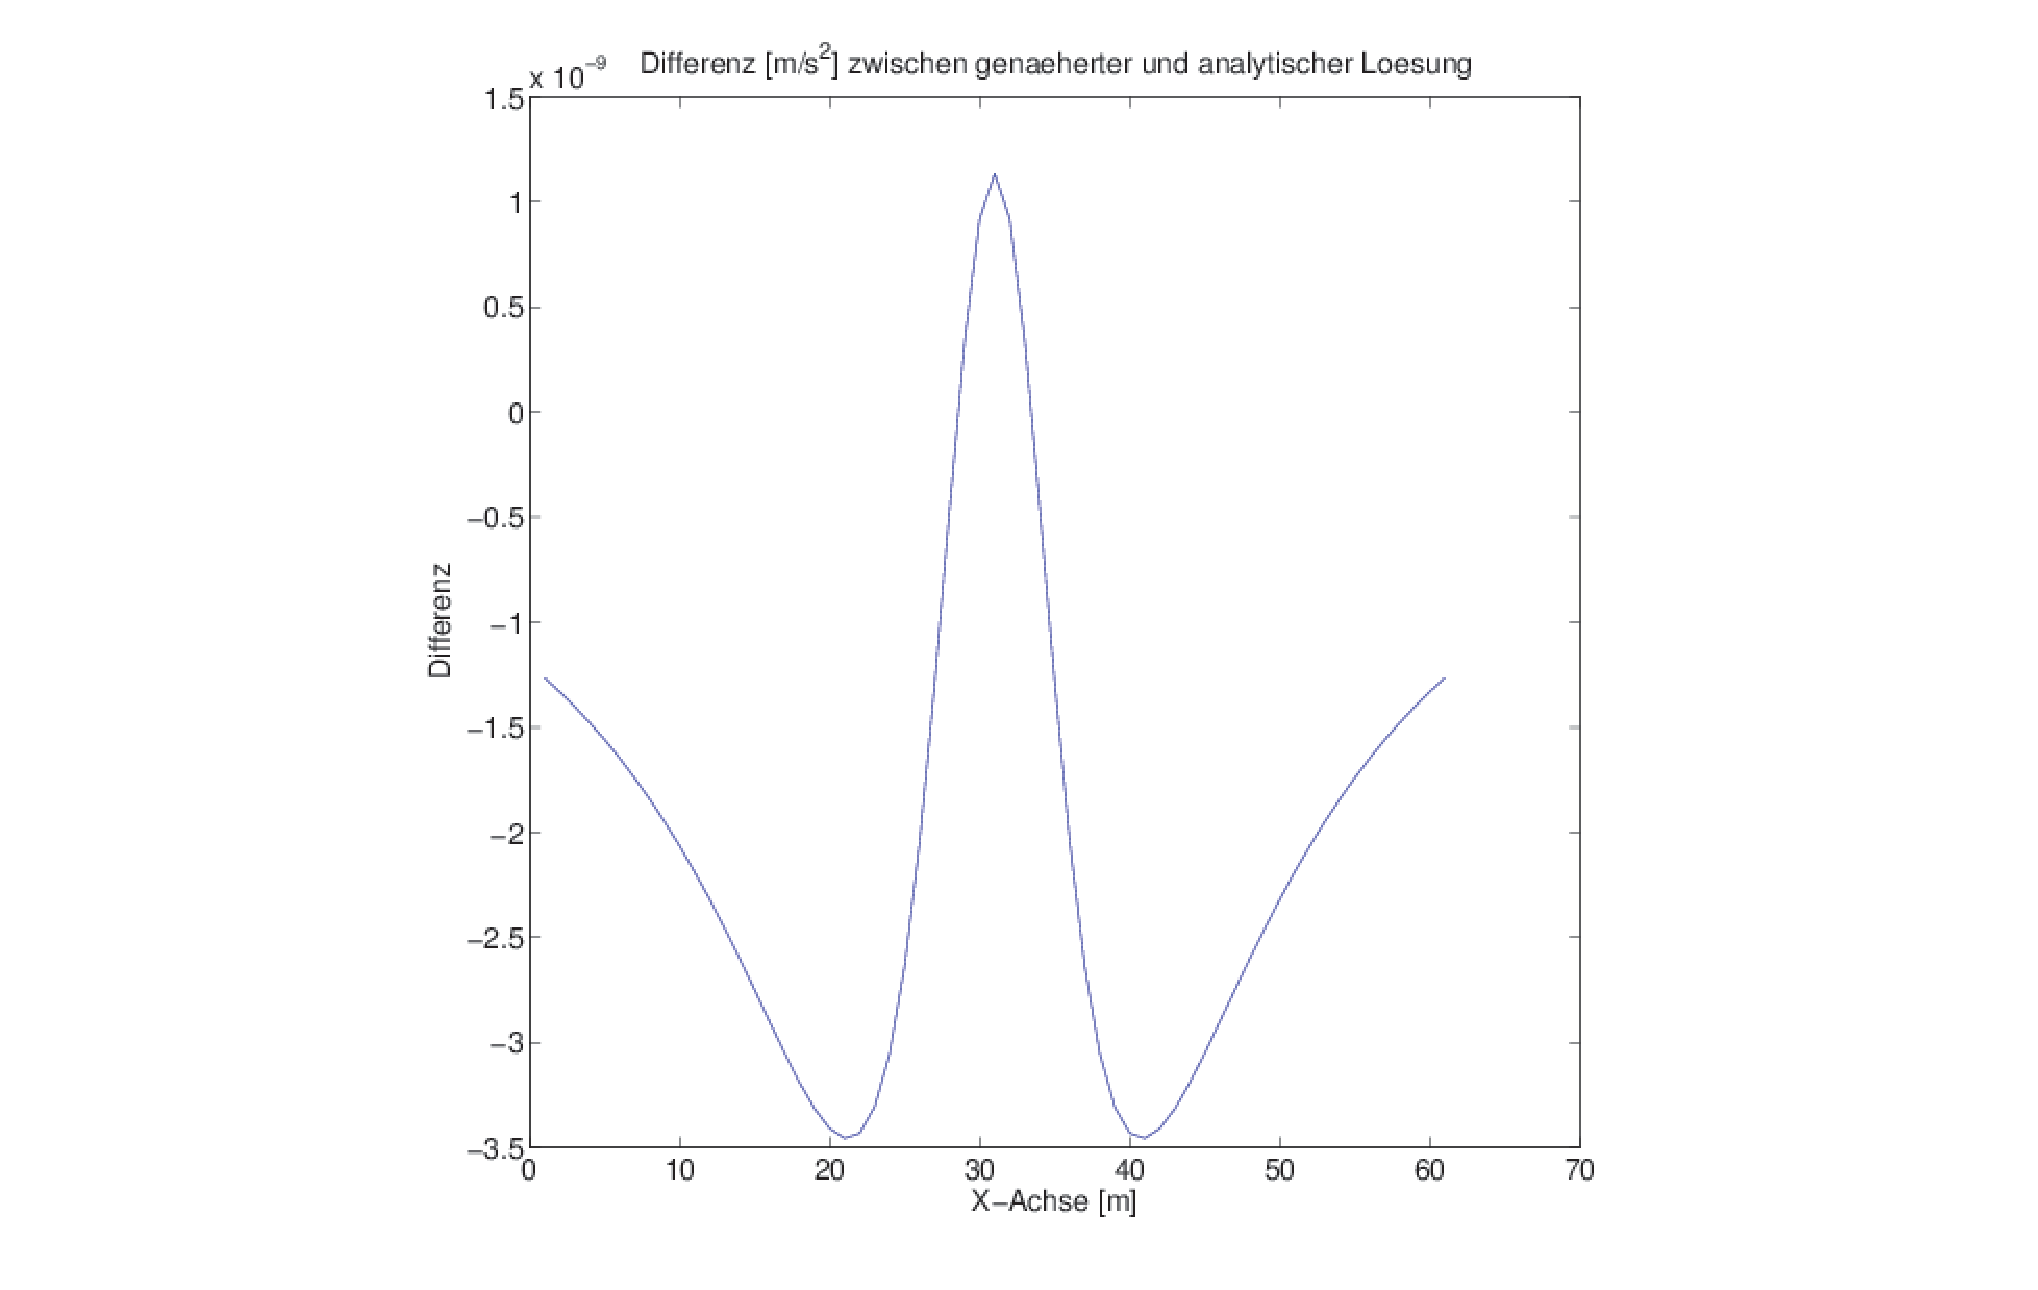
\includegraphics[scale=0.5]{Plots/DifferenzAnalytischApproximiert.pdf}
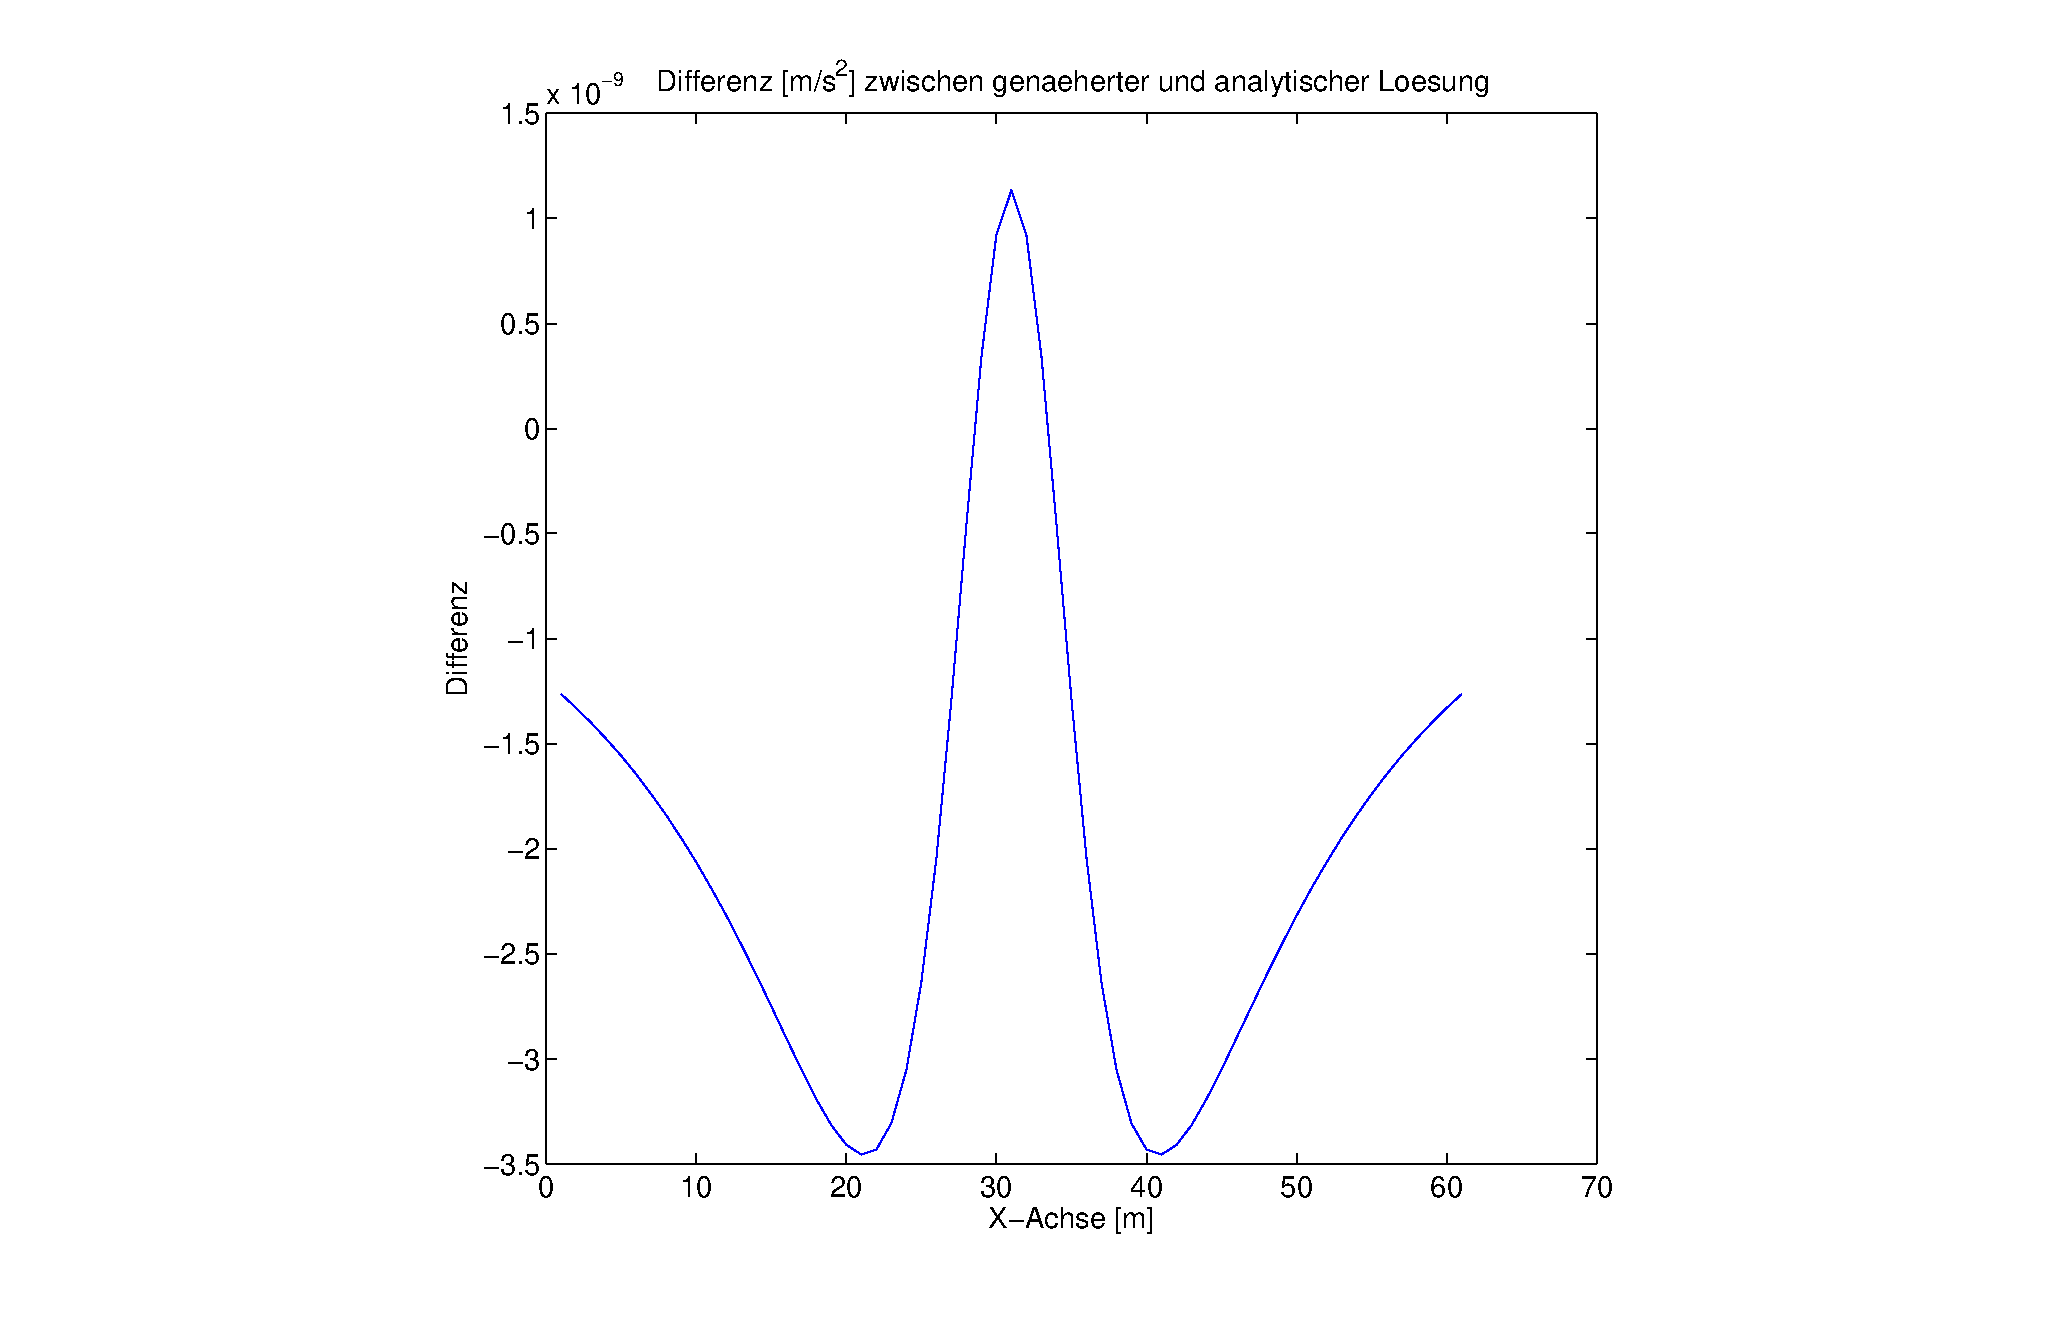
\includegraphics[scale=0.5]{Plots/DifferenzAnalytischApproximiert.eps}
\caption{Differenz zwischen analytischer L\"osung und N\"aherung bei x=0 und y=-15:15}
\label{fig:diff}
\end{center}
\end{figure}

% Das letzte Bild muss noch mal gemacht werden, da ist di Schrift wirklich schrecklich klein! K�nnt ihr das noch machen? Ich muss jetzt los!
